%------------------------------------------
% Fundamentos Teóricos
%------------------------------------------
\section{Fundamentos Teóricos}
\label{sec:fundamentos}


\todo[inline]{Aqui você vai apresentar os conceitos, as teorias, as técnicas e as tecnologias que sustentam a sua pesquisa e que são necessários para que a banca compreenda o problema e a solução proposta. No exame de qualificação, esta seção é um dos principais instrumentos para a banca avaliar o domínio do(a) mestrando(a) sobre a fundamentação do trabalho; portanto, vá além da simples definição de termos: discuta os conceitos com profundidade adequada ao nível de mestrado, compare abordagens alternativas e justifique as escolhas teóricas e tecnológicas adotadas. Por se tratar de um Mestrado Profissional em Computação Aplicada, articule a fundamentação com o domínio de aplicação (por exemplo, saúde, educação, agronegócio, gestão pública, indústria), apresentando também os conceitos essenciais desse domínio e, quando pertinente, normas técnicas, padrões e legislação aplicáveis (por exemplo, LGPD, normas ISO/IEC). Ao final de cada subseção, deixe explícito como o conceito apresentado será utilizado na solução proposta. Priorize fontes de qualidade, como livros de referência e artigos de periódicos e conferências relevantes na área, combinando referências clássicas com referências dos últimos cinco anos. Explique apenas o que é crucial para o seu trabalho e seja conciso. Evite citações literais longas e não use citações de citações (\textit{apud}).}


\subsection{Fundamentos 1}
\label{sec:fundamentos1}
\todo[inline]{Segue \textbf{um exemplo} de apresentação de código na linguagem de programação C que pode ser utilizado na apresentação de conceitos.}

\begin{figure}[thp]	
    \centering
    \begin{subfigure}{0.4\textwidth}
    \centering
    \begin{lstlisting}[language=C]       
double custo(double entrada)
{
  if (entrada < 0) 
  {
    return -1;
  }
  if ((entrada * 1.5) <= 0)) 
  {
    return -1;
  }
  if(entrada > 50) 
  {
    return 1.25*entrada;
  }
  return 1.5*entrada;
}
	\end{lstlisting}
    \caption{Código C}
  \end{subfigure}%    
  \begin{subfigure}{.05\textwidth}
    \hfill
  \end{subfigure}%    
  \begin{subfigure}{.4\textwidth}
    \centering
\begin{lstlisting}[language=C]   
TEST_CASE_1()
{
  double result;
  result = custo(0.49)
  assert(result == 0.735);
}
TEST_CASE_2()
{
  double result;
  result = custo(51)
  assert(result == 63.75);
}
\end{lstlisting}
  \caption{Código de Teste}
  \end{subfigure}%
  \caption{\label{fig:program_test} Exemplo de código}
\end{figure}


\subsection{Fundamentos 2}
\label{sec:fundamentos2}

\todo[inline]{Segue um exemplo de uso de figura}

A Figura~\ref{fig_grafico} apresenta uma imagem.

\begin{figure}[h!]    
	\begin{center}
	    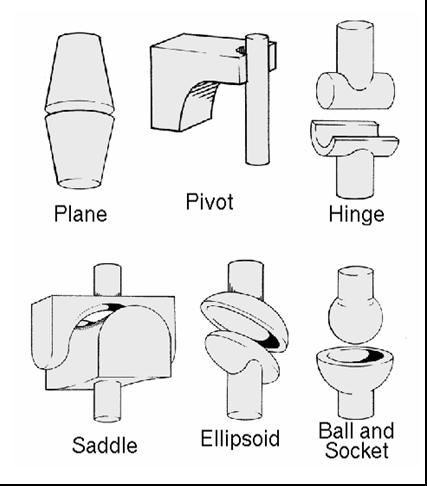
\includegraphics[scale=0.5]{imagens/fig2.jpg}
	\end{center}
    \caption{\label{fig_grafico}Descrição da imagem.}
\end{figure}

\subsection{Fundamentos 3}
\label{sec:fundamentos3}

\todo[inline]{Segue um exemplo de uso referências.}

Segundo \citeonline{knuth:84}, tem-se que $\dots$ \cite{boulic:91} e \cite{smith:99}.

\todo[inline]{Segue um exemplo de uso de referência de seção e de equações.}

Um exemplo de equação é apresentado na Equação~\ref{eq:poli}:

\begin{equation}
\label{eq:poli}
    f(n) = 4x^2 + 2y*12
\end{equation}

Outro exemplo de matemática em Latex: Calcule as raízes da equação $x^2 + 12x - 13 = 0$.
\begin{equation}
 x = \frac{-12 \pm \sqrt{12^2 - (4)(1)(-13)}}{(2)(1)} = \frac{-12 \pm \sqrt{196}}{2} = \frac{-12 \pm 14}{2} = -6 \pm 7
\end{equation}
